\documentclass[a4paper,11pt]{article}
\usepackage{setspace}
\usepackage{graphics}
\usepackage{geometry}
\usepackage{fancyhdr}
\usepackage{amsmath}
\usepackage{float,xeCJK}
\usepackage{amssymb}
\usepackage{listings}
\usepackage{xcolor}
\usepackage{fontspec}
\usepackage{enumerate}
\newfontfamily\couriernew{Courier New}
\lstset{
	backgroundcolor=\color[rgb]{0.9,0.9,0.9}, %设置背景颜色
    tabsize=4,    %tab大小
    language=[GNU]C++,
    basicstyle=\couriernew\small,	% 代码字体大小
    % basicstyle=\small,	% 代码字体大小
    upquote=true,
    aboveskip={1.5\baselineskip},
    columns=flexible,
    extendedchars=false,
    breaklines=true,
    % prebreak = \raisebox{0ex}[0ex][0ex]{\ensuremath{\hookleftarrow}},
    frame=single, % 代码加边框
    rulesepcolor=\color{white}, % 边框颜色
    numbers=left, % 行号的位置
    stepnumber=1, % 两个行号之间的差值
    numberstyle=\scriptsize\color[rgb]{0.205, 0.142, 0.73},% 行号大小 颜色
    numbersep=5pt, % 行号与代码间的距离
    showtabs=false, % 显示tab
    showspaces=false, %显示空格
    showstringspaces=false, %显示字符串中的空格
    identifierstyle=\ttfamily, %
    keywordstyle=\bfseries\color{blue},% 关键字颜色
    morekeywords={}, %增加关键字
    commentstyle=\color[rgb]{0,0.5,0}, % 注释颜色
    stringstyle=\color[rgb]{0.627,0.126,0.941},% 字符串颜色
    escapeinside={\%*}{*)}, % if you want to add LaTeX within your code
    % title=\lstname % 显示用\lstinputlisting导入的文件名
}

\setmonofont{Courier New}
\setCJKmainfont[BoldFont={Adobe Heiti Std}, ItalicFont={Adobe Kaiti Std}]{Adobe Song Std}
\setCJKmonofont{Courier New}
\linespread{1.3}
\setlength{\parindent}{2em}%首行  缩进
\geometry{left=2.5cm,right=2.5cm,top=2.5cm,bottom=2.5cm}
\addtolength{\parskip}{2pt} % 设置段间距
\renewcommand\figurename{图}

\begin{document}
\begin{center}
	\huge{\textbf{实验3 曲线拟合的最小二乘法\\}}
\end{center}
\begin{flushright}
	201311211914\\
	赵帅帅\\
	2016--5--10\\
\end{flushright}
\begin{Large}
	\textbf{一、 实验问题}
\end{Large}

	在某冶炼过程中,通过实验检测得到含碳量与时间关系的数据如下,试求含碳量y与时间t内在关系的拟合曲线。
	\begin{center}
		\begin{tabular}{c|ccccccccccc}
			\hline
			t & 0 & 5 & 10 & 15 & 20 & 25 & 30 & 35 & 40 & 45 & 50 \\
			\hline
			y & 0 & 1.27 & 2.16 & 2.86 & 3.44 & 3.87 & 4.15 & 4.37 & 4.51 & 4.58 & 4.02 \\
			\hline
		\end{tabular}
	\end{center}
\begin{Large}
	\textbf{二、 实验要求}
\end{Large}
\begin{enumerate}
	\item 用最小二乘法进行三次多项式的曲线拟合。
	\item 计算$y_i$与$y(t_j)$的误差,$j=1,2,\cdots,11$。
	\item 另取一个拟合函数,进行拟合效果的比较
	\item 绘制曲线拟合图形。
\end{enumerate}
\begin{Large}
	\textbf{三、 实验目的与意义}
\end{Large}
\begin{enumerate}
	\item 掌握曲线拟合的最小二乘法。
	\item 探求拟合函数的选择与拟合精度间的关系。
\end{enumerate}
\begin{Large}
	\textbf{四、 算法}
\end{Large}
	\begin{description}
		\item[输入 ] 自变量的值序列$x[N]$,观察函数值序列$y[N]$,每一组值的权重序列$\rho[N]$\footnote{本次实验$\rho[N]=\{1,1,\cdots,1\}$。},多项式拟合的最高次幂$M$。
		\item[输出 ] 拟合曲线的表达式。
	\end{description}
	\begin{enumerate}[(1)]
		\item 设置函数类$\Phi=span\{\boldsymbol{\varphi}_i(x)=x^i, 0\leqslant{}i\leqslant{}M\}$
		\item 引入向量
			\begin{eqnarray}
				\boldsymbol{\varphi}_j & = & (\boldsymbol{\varphi}_j(x_0),\boldsymbol{\varphi}_j(x_1),\cdots,\boldsymbol{\varphi}_j(x_{\scriptscriptstyle N-1}))^T,j=0,1,\cdots,M \nonumber\\
				\boldsymbol{f} & = & (y_0,y_1,\cdots,y_{\scriptscriptstyle N-1})^T \nonumber
			\end{eqnarray}		
			计加权内积
			\begin{eqnarray}
				(\boldsymbol{\varphi}_k,\boldsymbol{\varphi}_i) & = & \sum\limits_{j=0}^{N-1}\rho(x_j)\boldsymbol{\varphi}_k(x_j)\boldsymbol{\varphi}_i(x_j) \nonumber\\
				(\boldsymbol{f},\boldsymbol{\varphi}_i) & = & \sum\limits_{j=0}^{N-1}\rho(x_j)y_j\boldsymbol{\varphi}_i(x_j),k,i=0,1,\cdots,M \nonumber
			\end{eqnarray}
		\item 计算正则方程组
			\begin{displaymath}
				\left[
				\begin{array}{cccc}
				(\boldsymbol{\varphi}_0,\boldsymbol{\varphi}_0) & (\boldsymbol{\varphi}_0,\boldsymbol{\varphi}_1) & \cdots & (\boldsymbol{\varphi}_0,\boldsymbol{\varphi}_{\scriptscriptstyle M}) \\
			    (\boldsymbol{\varphi}_1,\boldsymbol{\varphi}_0) & (\boldsymbol{\varphi}_1,\boldsymbol{\varphi}_1) & \cdots & (\boldsymbol{\varphi}_1,\boldsymbol{\varphi}_{\scriptscriptstyle M}) \\
			    \vdots & \vdots & \ddots & \vdots \\
			    (\boldsymbol{\varphi}_{\scriptscriptstyle M},\boldsymbol{\varphi}_0) & (\boldsymbol{\varphi}_{\scriptscriptstyle M},\boldsymbol{\varphi}_1) & \cdots & (\boldsymbol{\varphi}_{\scriptscriptstyle M},\boldsymbol{\varphi}_{\scriptscriptstyle M}) \\
				\end{array}
				\right]\left[
				\begin{array}{c}
				a_0 \\ a_1 \\ \vdots \\ a_{\scriptscriptstyle M}
				\end{array}
				\right]=\left[
				\begin{array}{c}
				(\boldsymbol{f},\boldsymbol{\varphi}_0) \\ (\boldsymbol{f},\boldsymbol{\varphi}_0) \\ \vdots \\ (\boldsymbol{f},\boldsymbol{\varphi}_{\scriptscriptstyle M})
				\end{array}
				\right]
			\end{displaymath}
		\item 用平方根法或\textbf{SOR}迭代法解方程组得到$a=(a_0^*,a_1^*,\cdots,a_{\scriptscriptstyle M}^*)^T$
		\item 拟合曲线表达式$\boldsymbol{\varphi}^*(x)=a_0^*+a_1^*x+\cdots+a_{\scriptscriptstyle M}^{*}x^{\scriptscriptstyle M}$
	\end{enumerate}
\begin{Large}
	\textbf{五、 实验代码}
\end{Large}
\begin{spacing}{1.0}
	\begin{lstlisting}[language=C++]
#include<stdio.h>
#include<iostream>
#include<math.h>
#include<stdbool.h>
// M = 多项式最高次幂 + 1 
// N 为离散数据组数
const int M = 4, N = 11;
using namespace std;
double t[N] = {0, 5, 10, 15, 20, 25, 30, 35, 40, 45, 50};
double y[N] = {0, 1.27, 2.16, 2.86, 3.44, 3.87, 4.15, 4.37, 4.51, 4.58, 4.02};

// 点乘
double dot_product(double a[N], double b[N])
{
    double result = 0;
    for(int i = 0 ; i < N; i ++)
    {
        result += a[i] * b[i];
    }
    return result;
}

// 解正定线性方程组 from 实验1
bool Choleskey(double a[M][M], double b[M], double x[M])
{
    double sum = 0;
    double y[M] = {0};
    for(int k = 0; k <= M - 1; k ++)
    {
        sum = 0;
        for(int m = 0; m <= k - 1; m ++)
        {
            sum += a[k][m] * a[k][m];
        }
        a[k][k] = sqrt(a[k][k] - sum);
        if(a[k][k] == 0)
        {
            printf("Divided by zero!");
            return false;
        }
        for(int i = k + 1; i <= M - 1; i ++)
        {
            sum = 0;
            for(int m = 0; m <= k - 1; m ++)
            {
                sum += a[i][m] * a[k][m];
            }
            a[i][k] = (a[i][k] - sum) / a[k][k];
        }
        sum = 0;
        for(int m = 0; m <= k - 1; m ++)
        {
            sum += a[k][m] * y[m];
        }
        y[k] = (b[k] - sum) / a[k][k];
    }
    x[M - 1] = y[M - 1] / a[M - 1][M - 1];
    for(int k = M -2; k >= 0; k --)
    {
        sum = 0;
        for(int m = k + 1; m <= M - 1; m ++)
        {
            sum += a[m][k] * x[m];
        }
        x[k] = (y[k] - sum) / a[k][k];
    }
    return true;
}

int main(void)
{
    //
    double phi[M][N] = {0};
    for(int i = 0; i < M; i ++)
    {
        for(int j = 0; j < N; j ++)
        {
            phi[i][j] = pow(t[j], i);
        }
    }
    // 系数矩阵
    double a[M][M] = {0};
    // 值向量
    double b[M] = {0};
    // 待求解系数向量
    double x[M] = {0};
    for(int i = 0; i < M; i ++)
    {
        for(int j = 0; j < M; j ++)
        {
            a[i][j] = dot_product(phi[i], phi[j]);
        }
        b[i] = dot_product(y, phi[i]);
    }
    Choleskey(a, b, x);
    // 输出表达式
    cout<<"y = "<<x[0];
    for(int i = 1 ; i < M; i ++)
    {
        if(x[i] < 0)
            cout<<" - "<<fabs(x[i])<<"x^"<<i;
        else
            cout<<" - "<<x[i]<<"x^"<<i;
    }
    cout<<endl;
    // 输出误差
    for(int i = 0 ; i < N; i ++)
    {
        double result = 0;
        for(int j = 0; j < M; j ++)
        {
            result += x[j] * pow(t[i], j);
        }
        cout<<"y"<<i<<" - y"<<i<<"' = "<<y[i] - result<<endl;
    }
    return 0;
}

	\end{lstlisting}
\end{spacing}
\begin{Large}
	\textbf{六、实验结果}
\end{Large}
\begin{quote}
	\begin{description}
		\item[操作系统:] Windows 10 企业版
		\item[GCC 版本:] 4.7.1
		\item[G++ 版本:] 4.7.1
	\end{description}
\end{quote}
\begin{enumerate}
	\item 三次多项式拟合结果。
	\begin{figure}[H]
		\centering
		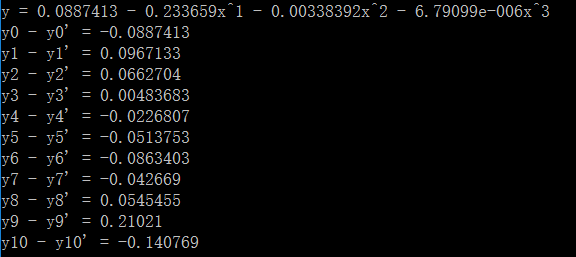
\includegraphics[width=12cm]{picture/result1.png}
		\caption{运行结果}
	\end{figure}
	\begin{figure}[H]
		\centering
		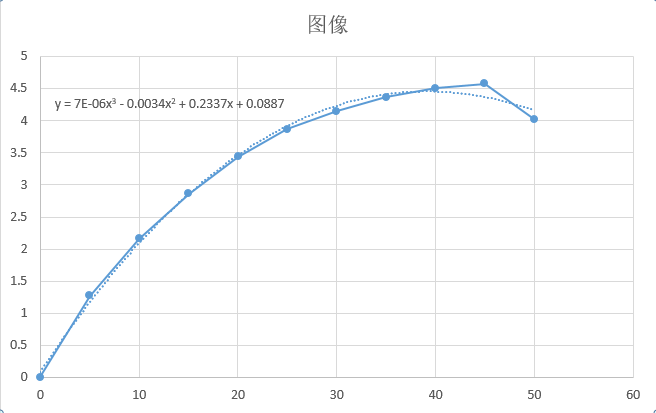
\includegraphics[width=12cm]{picture/image1.png}
		\caption{曲线图形}
	\end{figure}
	\item 另取一拟合函数拟合结果。\\
	取曲线拟合方程$y=ax^{\frac{1}{2}}+c$,变换关系为$\overline{x}=x^{\frac{1}{2}}$,得到变换的结果为$y=a\overline{x}+c$。\\
	程序运行结果如下:
	\begin{figure}[H]
		\centering
		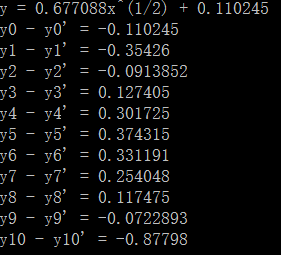
\includegraphics[width=8cm]{picture/result2.png}
		\caption{运行结果}
	\end{figure}
	\begin{figure}[H]
		\centering
		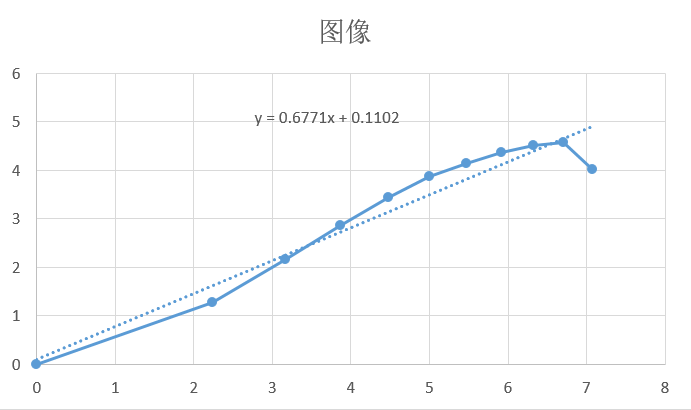
\includegraphics[width=12cm]{picture/image2.png}
		\caption{曲线图形(横轴为变量的平方根)}
	\end{figure}
	\item 两个拟合函数比较。\\
	直接观看两个拟合函数的拟合误差来看,多项式拟合效果较好。
\end{enumerate}
\begin{Large}
	\textbf{七、实验感受}
\end{Large}
\begin{enumerate}
	\item 本次实验需要我们自己抽象出代码所需要的算法,花了一点时间。
	\item 代码写起来还是很简单的。
\end{enumerate}
\end{document}